\documentclass{standalone}
\usepackage{tikz}
\usepackage{ctex,siunitx}
\setCJKmainfont{Noto Serif CJK SC}
\usepackage{tkz-euclide}
\usepackage{amsmath}
\usetikzlibrary{patterns, calc,3d}
\usetikzlibrary {decorations.pathmorphing,decorations.pathreplacing,decorations.shapes}
\renewcommand{\tabcolsep}{4pt}
\newcommand{\grids}[3]{\begin{tabular}{|c|c|c|} \hline #1 & #2 & #3 \\ \hline \end{tabular}}
\begin{document}
% \small
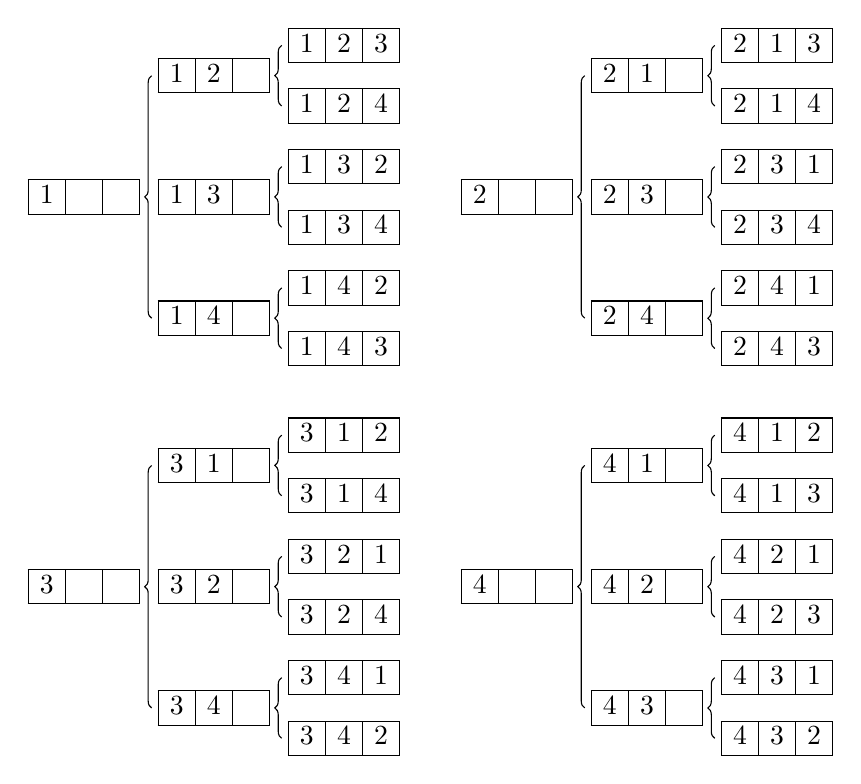
\begin{tikzpicture}[>=latex,scale=1.1,inner sep=0pt]
  \begin{scope}
    \node (n1) at (0,0)    {\grids{1}{2}{3}};
    \node (n2) at (0,-0.7) {\grids{1}{2}{4}};
    \node (n3) at (0,-1.4) {\grids{1}{3}{2}};
    \node (n4) at (0,-2.1) {\grids{1}{3}{4}};
    \node (n5) at (0,-2.8) {\grids{1}{4}{2}};
    \node (n6) at (0,-3.5) {\grids{1}{4}{3}};
    \draw [decorate,decoration={brace,raise=2pt}](n2.west)--(n1.west)node(n11)[midway,left=6pt]{\grids{1}{2}{\phantom{3}}};
    \draw [decorate,decoration={brace,raise=2pt}](n4.west)--(n3.west)node[midway,left=6pt]{\grids{1}{3}{\phantom{3}}};
    \draw [decorate,decoration={brace,raise=2pt}](n6.west)--(n5.west)node(n22)[midway,left=6pt]{\grids{1}{4}{\phantom{3}}};
    \draw [decorate,decoration={brace,raise=2pt}](n22.west)--(n11.west)node[midway,left=6pt]{\grids{1}{\phantom{3}}{\phantom{3}}};
  \end{scope}
  \begin{scope}[xshift=5cm]
    \node (n1) at (0,0)    {\grids{2}{1}{3}};
    \node (n2) at (0,-0.7) {\grids{2}{1}{4}};
    \node (n3) at (0,-1.4) {\grids{2}{3}{1}};
    \node (n4) at (0,-2.1) {\grids{2}{3}{4}};
    \node (n5) at (0,-2.8) {\grids{2}{4}{1}};
    \node (n6) at (0,-3.5) {\grids{2}{4}{3}};
    \draw [decorate,decoration={brace,raise=2pt}](n2.west)--(n1.west)node(n11)[midway,left=6pt]{\grids{2}{1}{\phantom{3}}};
    \draw [decorate,decoration={brace,raise=2pt}](n4.west)--(n3.west)node[midway,left=6pt]{\grids{2}{3}{\phantom{3}}};
    \draw [decorate,decoration={brace,raise=2pt}](n6.west)--(n5.west)node(n22)[midway,left=6pt]{\grids{2}{4}{\phantom{3}}};
    \draw [decorate,decoration={brace,raise=2pt}](n22.west)--(n11.west)node[midway,left=6pt]{\grids{2}{\phantom{3}}{\phantom{3}}};
  \end{scope}
  \begin{scope}[yshift=-4.5cm]
    \node (n1) at (0,0)    {\grids{3}{1}{2}};
    \node (n2) at (0,-0.7) {\grids{3}{1}{4}};
    \node (n3) at (0,-1.4) {\grids{3}{2}{1}};
    \node (n4) at (0,-2.1) {\grids{3}{2}{4}};
    \node (n5) at (0,-2.8) {\grids{3}{4}{1}};
    \node (n6) at (0,-3.5) {\grids{3}{4}{2}};
    \draw [decorate,decoration={brace,raise=2pt}](n2.west)--(n1.west)node(n11)[midway,left=6pt]{\grids{3}{1}{\phantom{3}}};
    \draw [decorate,decoration={brace,raise=2pt}](n4.west)--(n3.west)node[midway,left=6pt]{\grids{3}{2}{\phantom{3}}};
    \draw [decorate,decoration={brace,raise=2pt}](n6.west)--(n5.west)node(n22)[midway,left=6pt]{\grids{3}{4}{\phantom{3}}};
    \draw [decorate,decoration={brace,raise=2pt}](n22.west)--(n11.west)node[midway,left=6pt]{\grids{3}{\phantom{3}}{\phantom{3}}};
  \end{scope}
  \begin{scope}[xshift=5cm,yshift=-4.5cm]
    \node (n1) at (0,0)    {\grids{4}{1}{2}};
    \node (n2) at (0,-0.7) {\grids{4}{1}{3}};
    \node (n3) at (0,-1.4) {\grids{4}{2}{1}};
    \node (n4) at (0,-2.1) {\grids{4}{2}{3}};
    \node (n5) at (0,-2.8) {\grids{4}{3}{1}};
    \node (n6) at (0,-3.5) {\grids{4}{3}{2}};
    \draw [decorate,decoration={brace,raise=2pt}](n2.west)--(n1.west)node(n11)[midway,left=6pt]{\grids{4}{1}{\phantom{3}}};
    \draw [decorate,decoration={brace,raise=2pt}](n4.west)--(n3.west)node[midway,left=6pt]{\grids{4}{2}{\phantom{3}}};
    \draw [decorate,decoration={brace,raise=2pt}](n6.west)--(n5.west)node(n22)[midway,left=6pt]{\grids{4}{3}{\phantom{3}}};
    \draw [decorate,decoration={brace,raise=2pt}](n22.west)--(n11.west)node[midway,left=6pt]{\grids{4}{\phantom{3}}{\phantom{3}}};
  \end{scope}
\end{tikzpicture}
\end{document}